\def\QRCODE{TB_image_TUT.IMG.multiscale_matlabqrcode.png}
\def\QRPAGE{http://www.iptutorials.science/tree/master/TB_image/TUT.IMG.multiscale/matlab}
\mcorrectionsection{Matlab correction}

\subsection{Pyramidal decomposition and re\-cons\-truc\-tion}
\subsubsection{Decomposition}
The following function makes the decomposition of the Laplacian and Gaussian pyramids at the same time. The Laplacian pyramid can be reconstructed without any additional information. This is illustrated in Fig. \ref{fig:multiscale:matlab:glpyramid}.


\begin{matlab}
function [pyrG, pyrL] = LaplacianPyramidDecomposition(Image, levels, mode)
% Gaussian and Laplacian Pyramid decomposition
% Image must be either 2D (grayscale) or 3D (color)
% levels: number of levels of decomposition (not including the original level)
% mode: approximation mode 'bilinear', 'nearest', etc. for use in imresize
%       bilinear by default
% pyrG: Gaussian pyramid
% pyrL: Laplacian pyramid
%
% The Laplacian pyramid is of size levels+1. The last image pyrL{levels+1}
% is the approximation image of the last level. The original image is
% exactly reconstructed by the LaplacianPyramidReconstruction 
% function.

% pyramids
pyrL = cell(levels+1, 1);
pyrG = cell(levels+1, 1);

% gaussian filter
H = fspecial('gaussian');

if ~exist('mode', 'var')
    mode = 'bilinear';
end

for i=1:levels
    ImagePrec = Image; % previous image
    g=imfilter(Image,H,'same');
    
    Image = imresize(g, .5, mode);
    ImagePrime = imresize(Image, [size(g,1), size(g,2)], mode);
    
    pyrL{i} =  ImagePrec - ImagePrime;
    pyrG{i} =  ImagePrec;

end
pyrL{levels+1} = Image;
pyrG{levels+1} = Image;
\end{matlab}

\begin{mcomment}
\begin{mremark}
Notice that the images are of type double, which implies a special care when displaying them, for example by using the command \minline{imshow(I, [])}.
\end{mremark}
\end{mcomment}



\begin{figure}[htbp]
\centering
 \subfloat[Original image.]{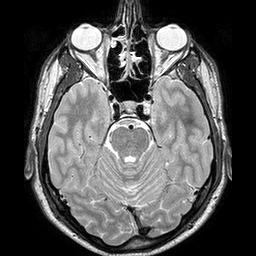
\includegraphics[width=.5\linewidth]{cerveau.jpg}}
 
 \subfloat[Gaussian pyramid le\-vel 1.]{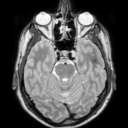
\includegraphics[width=.3\linewidth]{pyrG2.png}}\hfill
 \subfloat[Level 2.]{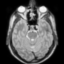
\includegraphics[width=.3\linewidth]{pyrG3.png}}\hfill
 \subfloat[Level 3.]{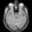
\includegraphics[width=.3\linewidth]{pyrG4.png}}

 \subfloat[Laplacian pyramid le\-vel 1.]{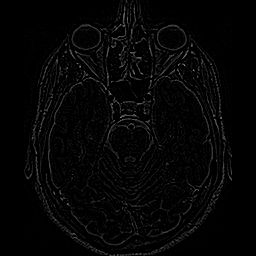
\includegraphics[width=.3\linewidth]{pyrL1.png}}\hfill
 \subfloat[Level 2.]{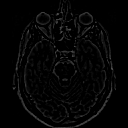
\includegraphics[width=.3\linewidth]{pyrL2.png}}\hfill
 \subfloat[Level 3.]{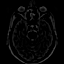
\includegraphics[width=.3\linewidth]{pyrL3.png}}
 \caption{Gaussian and Laplacian pyramids, for 3 levels of decomposition. The Laplacian pyramid in addition to the last level of the Gaussian pyramid is required to exactly reconstruct the original image.}
 \label{fig:multiscale:matlab:glpyramid}
\end{figure}

\subsubsection{Reconstruction}
The reconstruction is straighforward and exact because of the construction of the residue. The details can be filtered (removed for example), thus giving the following result Fig. \ref{fig:multiscale:matlab:nodetails}.

\begin{matlab}
function Image = LaplacianPyramidReconstruction(pyr, mode)
% Laplacian Pyramid Reconstruction
% pyr: Laplacian pyramid
% mode: approximation mode for imresize, bilinear by default

if ~exist('mode', 'var')
    mode = 'bilinear';
end

levels = size(pyr, 1)-1;

Image = pyr{levels+1};
% reconstruction from bottom to top
for i=levels:-1:1
    Image = pyr{i} + imresize(Image, ...
                     [size(pyr{i},1), size(pyr{i}, 2)], mode);
end
\end{matlab}

\begin{figure}[htbp]
\centering
 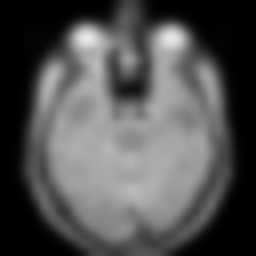
\includegraphics[width=4cm]{nodetails.png}
 \caption{Reconstruction of the pyramid without any detail.}
 \label{fig:multiscale:matlab:nodetails}
\end{figure}


\subsection{Scale-space decomposition and multiscale filtering}
\begin{matlab}
% Morphological scale-space decomposition 
k=3; % number of decompositions
ss=cell(2,k);
for i=1:k
    se = strel('disk',2*i); % structuring element
    ss{1,i}=imdilate(A,se); % dilation
    ss{2,i}=imerode(A,se);  % erosion
end
\end{matlab}


\begin{figure}[htbp]
\centering
 \subfloat[Dilation scale 1.]{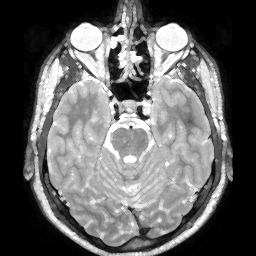
\includegraphics[width=.3\linewidth]{pyrdil1.png}}\hfill
 \subfloat[Dilation scale 2.]{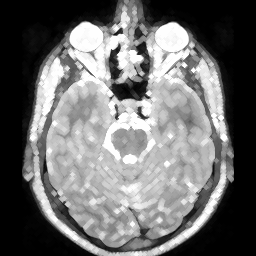
\includegraphics[width=.3\linewidth]{pyrdil2.png}}\hfill
 \subfloat[Dilation scale 3.]{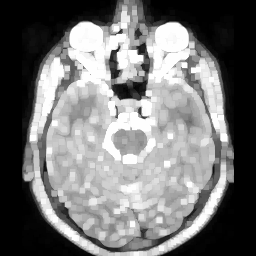
\includegraphics[width=.3\linewidth]{pyrdil3.png}}
 \caption{Morphological multiscale decomposition by dilation.}
 \label{fig:multiscale:matlab:dilation}
\end{figure}

\begin{figure}[htbp]
\centering
 \subfloat[Erosion scale 1.]{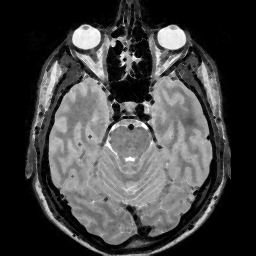
\includegraphics[width=.3\linewidth]{pyrero1.png}}\hfill
 \subfloat[Erosion scale 2.]{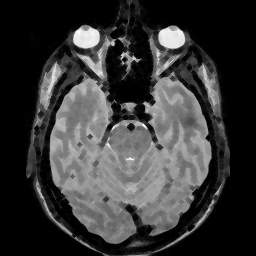
\includegraphics[width=.3\linewidth]{pyrero2.png}}\hfill
 \subfloat[Erosion scale 3.]{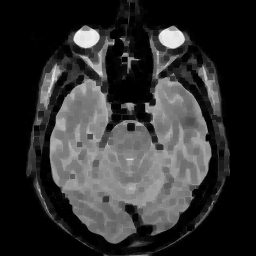
\includegraphics[width=.3\linewidth]{pyrero3.png}}
 \caption{Morphological multiscale decomposition by erosion.}
 \label{fig:multiscale:matlab:erosion}
\end{figure}

\subsection{Kramer and Bruckner multiscale decomposition}
The results are illustrated in Fig.\ref{fig:multiscale:matlab:KB}.

\begin{figure}[htbp]
\centering
 \subfloat[$MK_{B}^1$.]{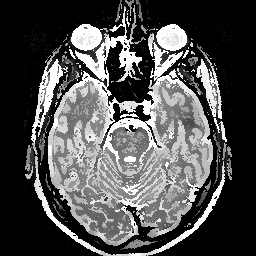
\includegraphics[width=.3\linewidth]{mkb1.png}}\hfill
 \subfloat[$MK_{B}^2$.]{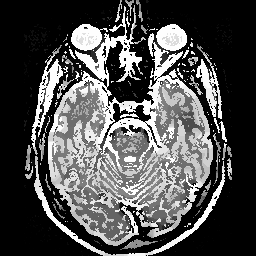
\includegraphics[width=.3\linewidth]{mkb2.png}}\hfill
 \subfloat[$MK_{B}^3$.]{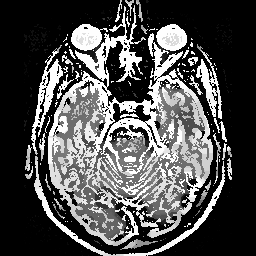
\includegraphics[width=.3\linewidth]{mkb3.png}}

 \caption{Kramer and Bruckner multiscale decomposition, for $r=5$.}
 \label{fig:multiscale:matlab:KB}
\end{figure}

\begin{matlab}
sskb=cell(1,k+1);
sskb{1, 1} = A;
r  = 5;
for i=2:k+1
   sskb{1,i}=kb(sskb{1,i-1}, r);
end
\end{matlab}

\begin{matlab}
function K = kb(I, r)
% Kramer and Bruckner iterative filter
% I: originale image
% r: size of neighborhood
%
% return filtered image
se = strel('disk', r);
D = imdilate(I, se);
E = imerode(I, se);
difbool=double((D-I)<(I-E));

K = D.*difbool+E.*(1-difbool); 
\end{matlab}
